% begin module natural-growth-population-Ex
\begin{frame}
\begin{example}
Use the fact that the world population was 2560 million in 1950 and 3040 
million in 1960 to model the population of the world in the second 
half of the 20th century. \\
(Assume the growth rate is proportional to the population size.) \\

What is the relative growth rate? \\

Use the model to estimate the world population in 1993 and to predict the
 population in the year 2020.
\end{example}
\textbf{SOLUTION:}\\ \pause 
We measure the time $t$ in years and let $t = 0$ in the year 1950.\\ \pause
We measure the population $P(t)$ in millions of people. 
Then $P (0) = 2560$ and $P (10) = 3040$.
\\ \pause 
Since we are assuming that $\frac{dP}{dt} = kP$, the Theorem gives
 \[
P(t) = P(0)e^{kt} = 2560e^{kt}
\]      \pause   
Now find the relative growth rate, $k$:\\
$\ds  P(10) = 2560e^{10k}=3040 \pause\;\; \To\;\;  e^{10k}=\frac{3040}{2560}=\frac{19}{16}
 $
\end{frame}
\begin{frame}
take the logarithm of both sides \pause
$ e^{10k}=\frac{19}{16} \To\;\; 10k=\ln\left(\frac{19}{16}\right)\;\;$ \pause $\To\;\; k = \frac{1}{10}\ln\left(\frac{19}{16}\right)$\pause $ \;\; = \ln\left(\frac{19}{16}\right)^\frac{1}{10}$\pause $ \approx 0.017185$ \\ \pause 
So the relative growth rate is about 1.7\% per year and the model is
\begin{align*}
P(t) & =2560e^{kt}=2560e^{\frac{t}{10}\ln(19/16)}= 2560e^{\ln\left( 19/16 \right)^{\frac{t}{10}}}\\ 
& = 2560\cdot \left(\frac{19}{16}\right)^\frac{t}{10}
\end{align*}\pause
According to this model, the estimated  world population in 1993 was
\[
P(43)= 2560\cdot \left(\frac{19}{16}\right)^\frac{43}{10}\approx 5360 \text{ (million)}
\]
\pause
The model predicts that the population in 2020 will be
\[
P(70)= 2560\cdot \left(\frac{19}{16}\right)^7\approx 8525 \text{ (million)}
\]
\end{frame}
\begin{frame}
\begin{figure}
\centering
\caption{The graph shows that the model is fairly accurate to the end of the 20th century (the dots represent the actual population), so the estimate for 1993 is quite reliable. But the prediction for 2020 is riskier.}
\label{fig:World}
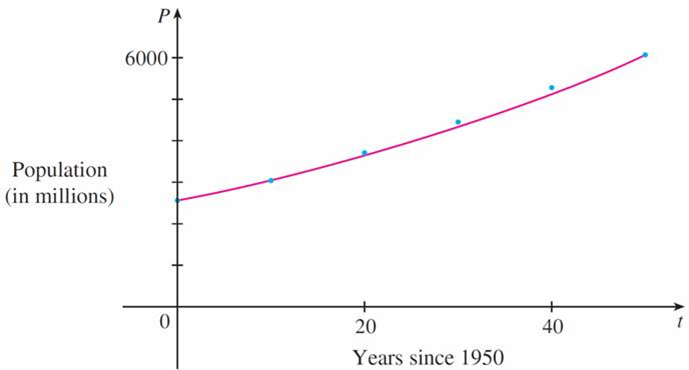
\includegraphics[width=0.7\linewidth]{../../modules/exponential-growth-and-decay/pictures/World}
\end{figure}

\end{frame}
% end module natural-growth-population-Ex
